% --------------------------------------------------------------------------------------
% DOCUMENT METADATA - TO BE FILLED BY USER
% --------------------------------------------------------------------------------------
% --- Document Type ---
\newcommand{\DocumentType}{TEST REPORT}    

% --- Project Identification ---
\newcommand{\ProjectRef}{25P01}                     
\newcommand{\ProjectTitle}{MORSE KEY}              

% --- Report Identification ---
\newcommand{\ReportRef}{R02}                           
\newcommand{\ReportTitle}{EXPERIMENTAL DESIGN VALIDATION} 
\newcommand{\DocVersion}{V01}                           

% --- Authoring and Assets ---
\newcommand{\AuthorName}{Nick McCleery}
\newcommand{\ReleaseDate}{\today}             
\newcommand{\LogoPath}{./assets/logo.pdf}     
\newcommand{\ReferenceFile}{25P01-R02V01-ExperimentalDesignValidation.bib} 
% --------------------------------------------------------------------------------------
% END DOCUMENT METADATA
% --------------------------------------------------------------------------------------

% --------------------------------------------------------------------------------------
% DOCUMENT SETUP — GENERALLY TO BE LEFT UNCHANGED
% --------------------------------------------------------------------------------------
% Assemble shorthand
\newcommand{\ProjectFullRef}{\ProjectRef{} \ProjectTitle{}}
\newcommand{\ReportFullRef}{\ReportRef{}-\DocVersion{}}

% Fonts
\documentclass[10pt]{article}

\usepackage[utf8]{inputenc}
\usepackage[OT1]{fontenc}
\usepackage{ocr}

\usepackage{lmodern}
\renewcommand*\familydefault{\sfdefault}

% Set sections to use OCR-A1
\usepackage{sectsty}
\sectionfont{\ocrfamily\Large}
\subsectionfont{\ocrfamily\large}
\subsubsectionfont{\ocrfamily\normalsize}

% Core packages
\usepackage[english]{datetime2}
\usepackage{amsmath}
\usepackage{amssymb}
\usepackage{array}
\usepackage{booktabs}
\usepackage{enumitem}
\usepackage{fancyhdr}
\usepackage{float}
\usepackage{geometry}
\usepackage{graphicx}
\usepackage{longtable}
\usepackage{textcomp}
\usepackage{titlesec}
\usepackage{titling}
\usepackage{xcolor}

% Links
\usepackage[colorlinks=true,
            linkcolor=gray,
            citecolor=gray,
            urlcolor=gray
           ]{hyperref}

% Date
\DTMsetdatestyle{iso}

% Bibliography
\usepackage[backend=bibtex, style=ieee, citestyle=numeric-comp]{biblatex}
\addbibresource{\ReferenceFile}


% Set narrow page margins
\geometry{
  paper=a4paper,
  top=0.75in,
  bottom=0.75in,
  left=0.55in,
  right=0.55in,
  headsep=0.25in
}

% Remove paragraph indentation, add spacing between paragraphs
\usepackage{parskip}
\setlength{\parindent}{0pt}
\setlength{\parskip}{6pt}

% Header/Footer setup
\pagestyle{fancy}
\fancyhf{}
\renewcommand{\headrulewidth}{0.4pt}
\renewcommand{\footrulewidth}{0pt}
\fancyfoot[C]{\thepage}
\fancyhead[L]{\ocrfamily\small\ProjectFullRef}
\fancyhead[R]{\ocrfamily\small\ReportFullRef}
\setlength{\headheight}{20pt}

% Custom section style with horizontal lines
\titleformat{\section}
  {\ocrfamily\Large\bfseries}
  {\thesection}{1em}{}
  \titlespacing*{\section}
  {0pt}{1.5em}{1em}

\titleformat{\subsection}
  {\ocrfamily\large\bfseries}
  {\thesubsection}{1em}{}

\titleformat{\subsubsection}
  {\ocrfamily\normalsize\bfseries}
  {\thesubsubsection}{1em}{}

% Create a custom title command
\newcommand{\customtitle}{%
  \noindent
  \begin{minipage}[t]{0.65\textwidth}
    \vspace{-0.5cm}
    {\ocrfamily\Large\bfseries \DocumentType \par}
  \end{minipage}%
  \begin{minipage}[t]{0.35\textwidth}
    \flushright{}
    \includegraphics[width=0.5\textwidth]{\LogoPath}
  \end{minipage}

  \vspace{0.3cm}
  \hrule height 0.8pt
  \vspace{0.3cm}

  {\ocrfamily\bfseries\ProjectFullRef\par}
  {\ocrfamily\large\bfseries\ReportTitle\par}

  \vspace{0.5em}

  \begin{tabular}{@{}ll@{\hspace{2cm}}ll@{}}
    \ocrfamily\textbf{REPORT REF:} & \ocrfamily \ReportRef &
    \ocrfamily\textbf{AUTHOR:}     & \ocrfamily \AuthorName \\

    \ocrfamily\textbf{VERSION:}    & \ocrfamily \DocVersion &
    \ocrfamily\textbf{DATE:}       & \ocrfamily \ReleaseDate \\
  \end{tabular}

  \vspace{0.3cm}
  \hrule height 0.8pt
  \vspace{0.25cm}
}

% Create fullwidth table command
\newenvironment{fullwidthtable}
  {\begin{center}
   \begin{tabular*}{\textwidth}{@{\extracolsep{\fill}}ll@{}}}
  {\end{tabular*}
   \end{center}}


% Fold URLs
\usepackage{xurl}
\setlength{\emergencystretch}{1em}

\begin{document}
\vspace*{-1cm}
\thispagestyle{plain}
\customtitle{}

% --------------------------------------------------------------------------------------
% BEGIN REPORT CONTENT
% --------------------------------------------------------------------------------------
\section{Summary}

This document describes the experimental procedure used to validate the design of a simple flexure
hinge Morse key.

Testing demonstrated a measured stiffness of 0.37N/mm, within 5.1\% of the
analytical prediction. Given the known limitations of the prediction methods, this is considered to
validate the design approach for the flexure hinge.

\section{Objectives}

The aim of the work was to examine the basic force-displacement characteristic of the key under
static load, ultimately allowing for comparison of measured key stiffness with analytical
predictions.

\section{Equipment}

Ideally, the Morse key would be mechanically characterised with a servohydraulic load frame,
allowing for the controlled application of target force and measurement of the corresponding
resultant displacement, or vice versa. However, without access to dedicated mechanical testing
equipment, an improvised test rig was constructed using a 3D printer, digital kitchen scales, and a
fastener of known pitch.

The test rig shown in \autoref{fig:gantry-rig} consists of a 3D printed gantry frame with an
M12x1.75 fastener serving as a vertical lead screw. As the screw is rotated, it compresses the
Morse key, which is located on inexpensive digital scales. Displacement is calculated from the
screw's thread pitch and angular displacement, while the scales measure the resulting force
response. This arrangement allows for rough force-displacement characterisation without specialised
equipment

\begin{figure}[H]
	\centering
	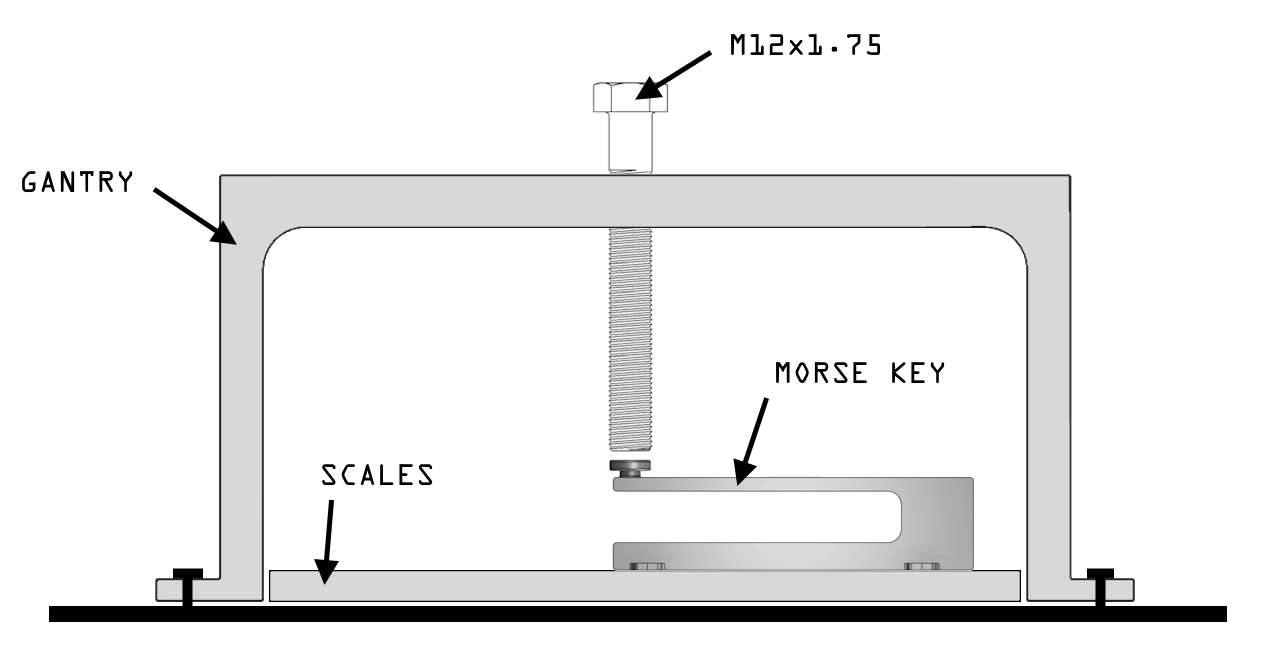
\includegraphics[width=0.75\textwidth]{./assets/GantryArrangement.png}
	\caption{Gantry Rig Arrangement}
	\label{fig:gantry-rig}
\end{figure}

\begin{figure}[H]
	\centering
	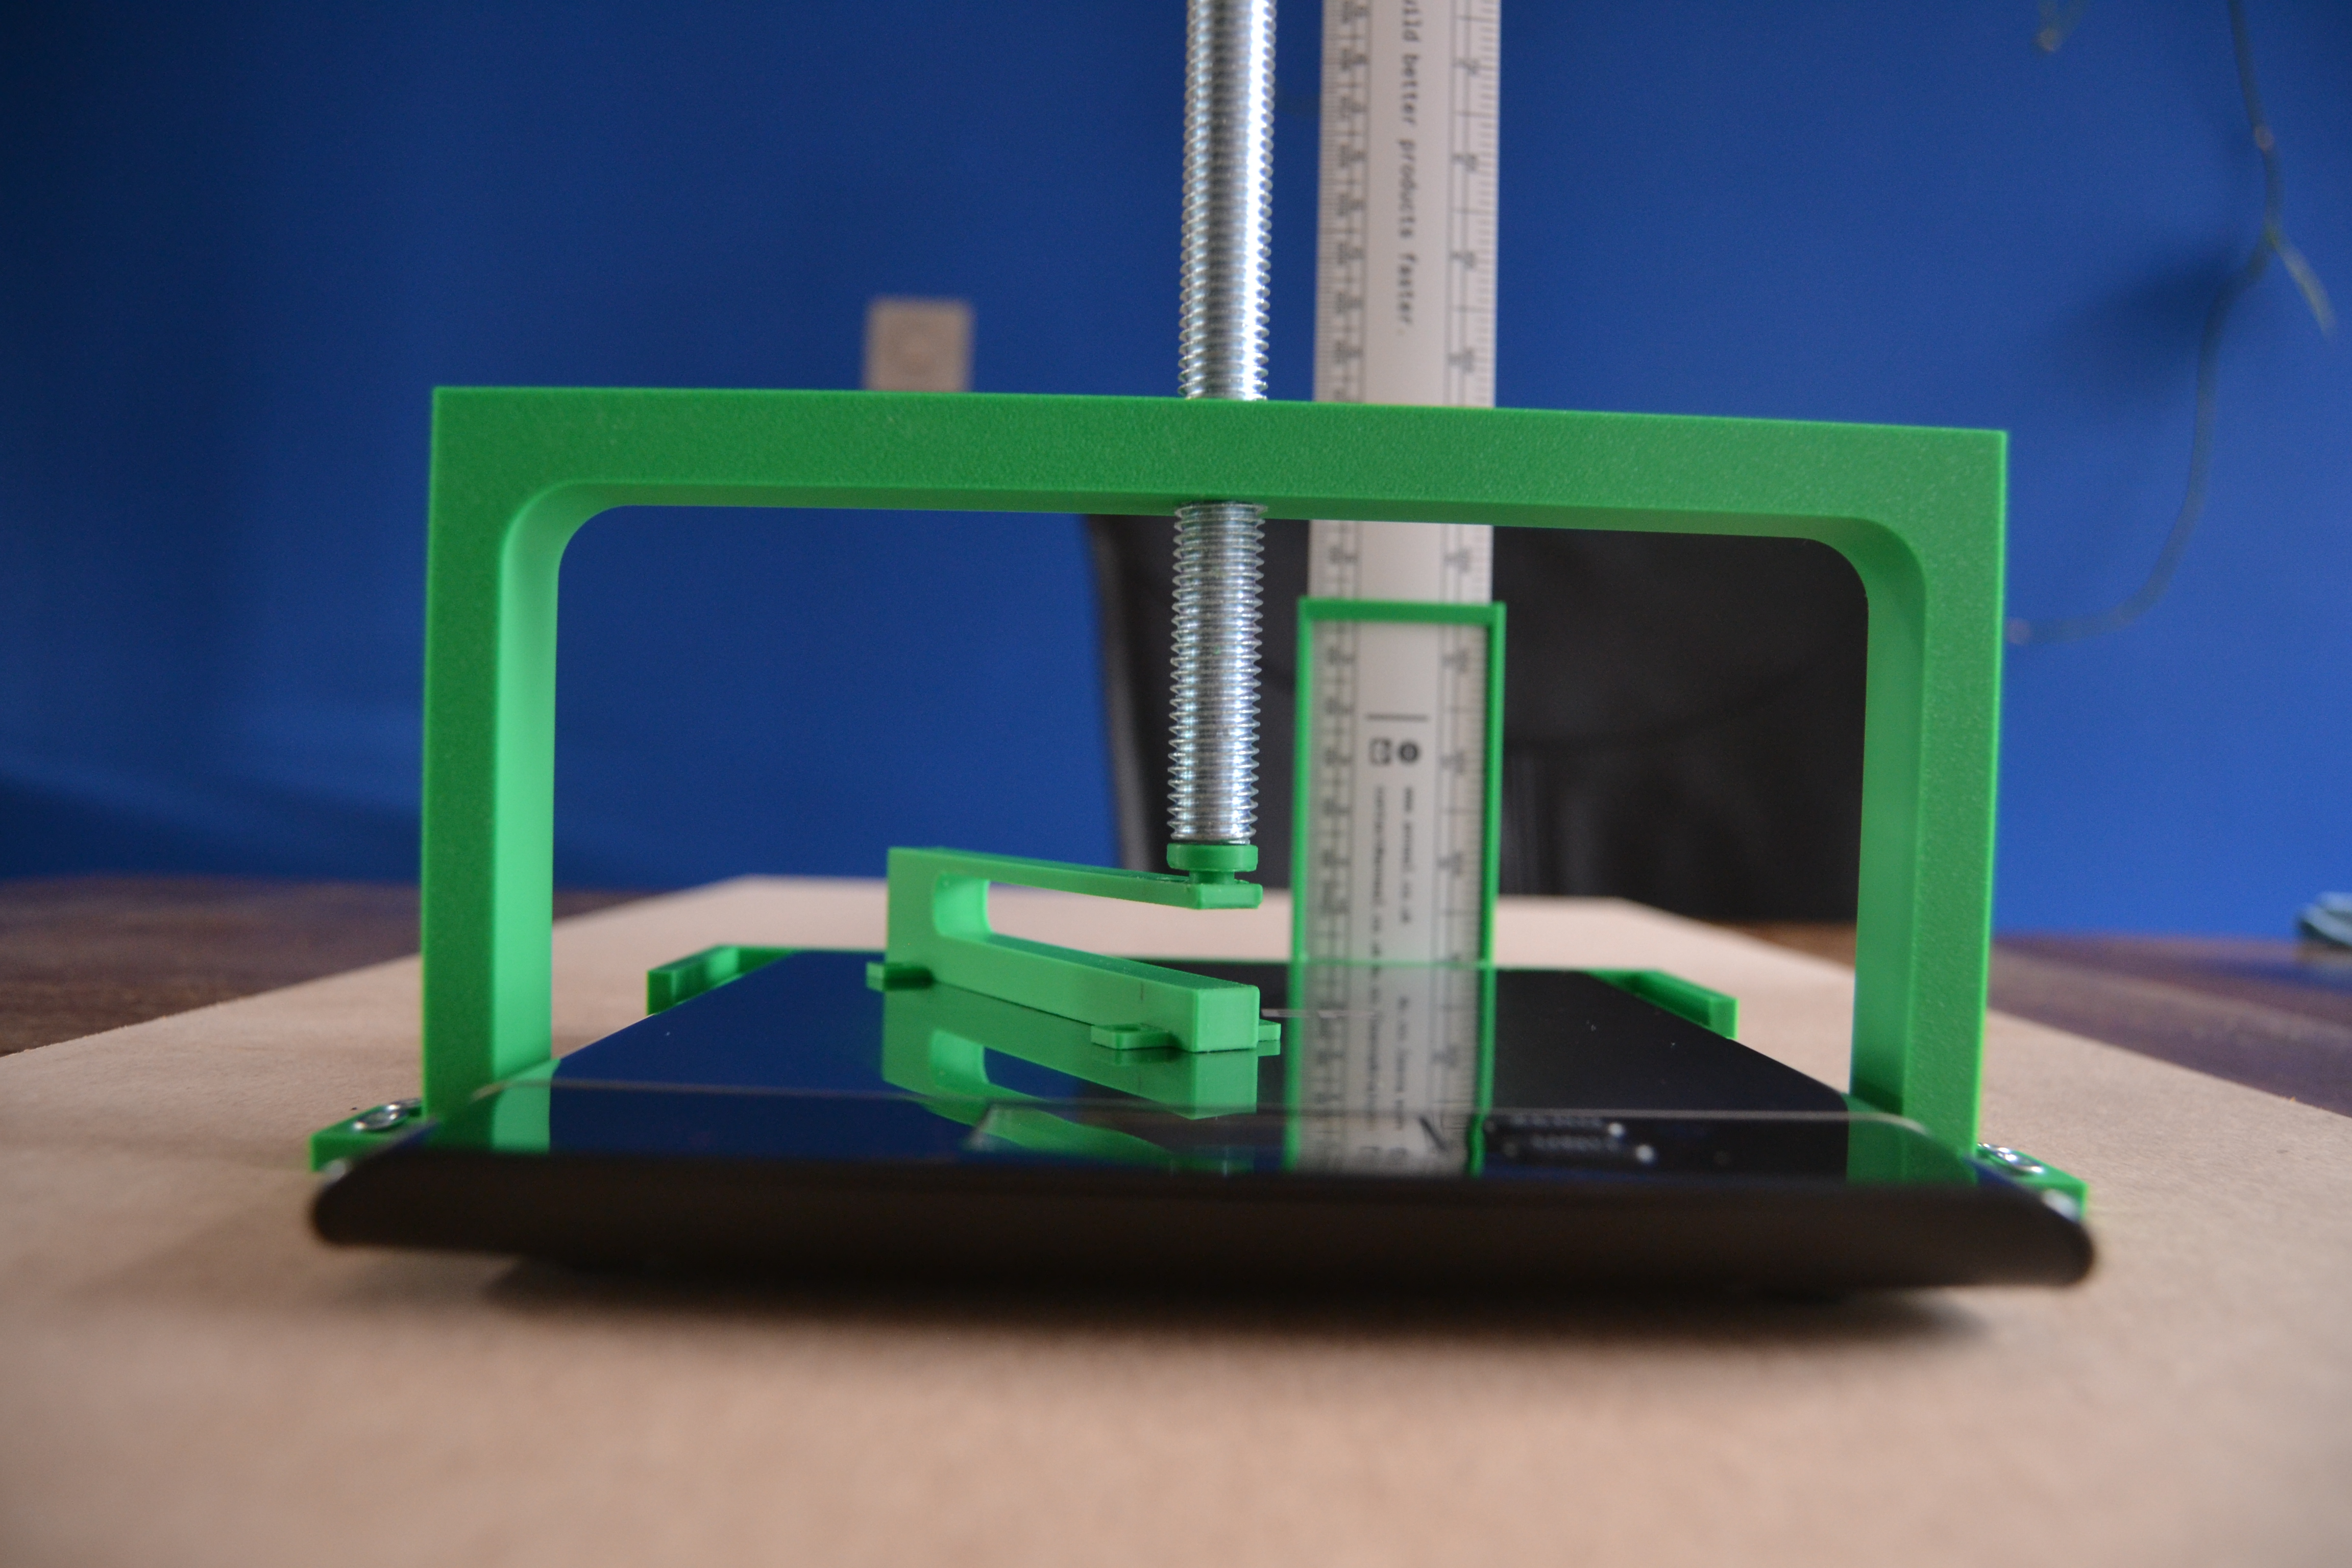
\includegraphics[width=0.75\textwidth]{./assets/DSC_0001.JPG}
	\caption{Gantry Rig Arrangement, Assembled}
	\label{fig:gantry-rig-photo}
\end{figure}

\section{Method}

The experimental procedure adopted was as follows:
\begin{enumerate}
	\item The Morse key was positioned under the gantry and the scales were zeroed.
	\item The lead screw was advanced until initial contact with the key was confirmed by a low magnitude
	      reading on the scales; around 1-2g.
	\item The screw was backed off until the scales returned to 0g indicated, and the screw head was marked
	      in the `zero position' with a permanent marker.
	\item The screw was then rotated in 180° increments, with force readings recorded at each step.
\end{enumerate}

\section{Results}

Results are given in \autoref{fig:results}. The data is presented as a force-displacement plot,
with target stiffness values also indicated.

Results show that the measured stiffness of the key is approximately 0.37N/mm, $r^2=0.98$. The
testing covered a force range from 0gf to 170gf (approximately 1.67N), sufficient to characterise
the key's operating range. Throughout this range, the response remained largely linear, with
deviations assumed to be primarily a function of the lack of locating features for the key within
the test rig. The key was free to move in the horizontal plane, which may have given rise to error.

Given that predicted/target stiffness was 0.39N/mm, the results indicate an error of 5.1\%. Given
the rudimentary nature of the test rig and the known limitations of the prediction methods, this
was considered an acceptable result, and one that largely validates the approach used in the design
phase.

\begin{figure}[H]
	\centering
	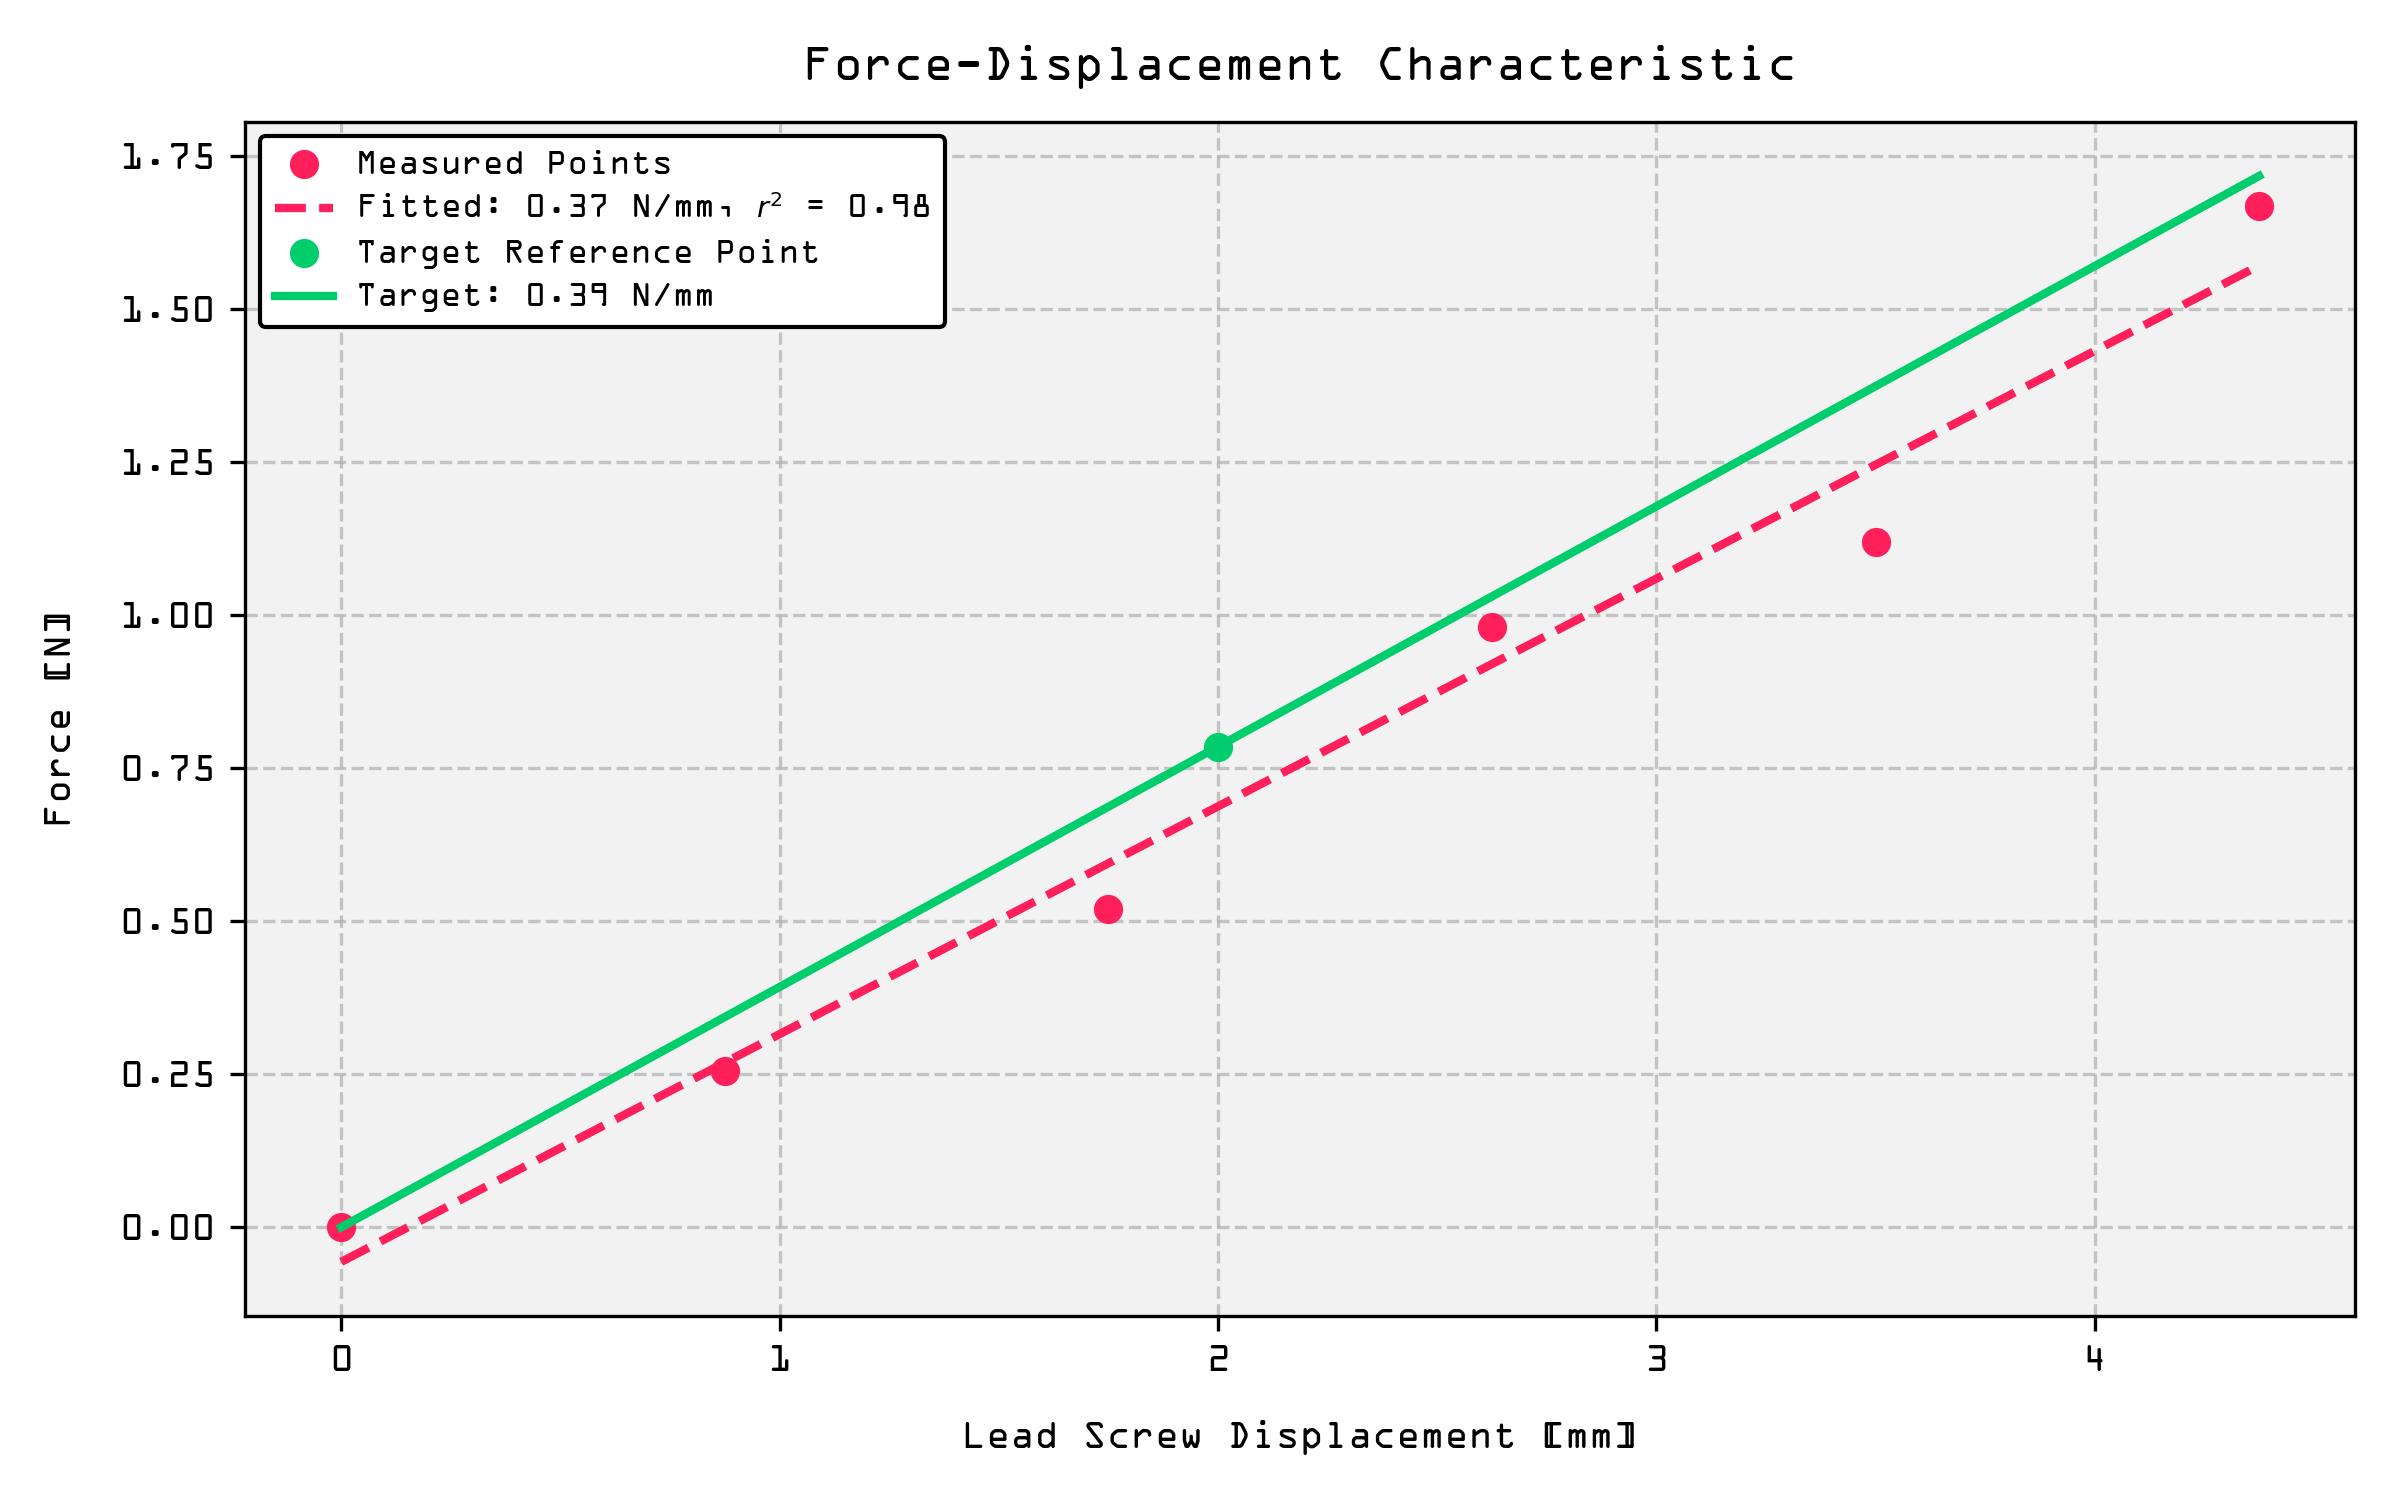
\includegraphics[width=0.75\textwidth]{./assets/09-test-results.png}
	\caption{Test Results}
	\label{fig:results}
\end{figure}

% \section{References}
% \printbibliography[heading=none]

\end{document}